\chapter{Polar Coordinate System}
\label{cha:polar-coord-syst}
\lecture{1}{9 Apr. 14:00}{Polar Coordinate System}

\section{Setting up a Polar Coordinate System}
\label{sec:polar-coord-syst}

To setup a polar coordinate system, we need a \textbf{pole}(origin) and a
reference direction called \textbf{polar axis} usually in the direction of the
+ve x-axis in the cartesian coordinate plane.


\begin{note}[Polar Coordinates]
  Polar Coordinates help you to locate a point using a distance and an angle.
  \begin{enumerate}
    \item \textbf{Radial Coordinate \( (r) \) } This is the distance from a
      fixed reference point, known as the pole (or origin), to the point in
      question.
    \item \textbf{Angular Coordinate \( (\theta) \)} This is the angle between
      the line connecting the pole to the point and a reference direction,
      typically the positive x-axis, measured counterclockwise.
  \end{enumerate}

  The polar coordinates of a point are denoted as \( (r,\theta) \).
\end{note}

\section{Uniqueness of Polar Coordinates}
\label{sec:uniq-polar-coord}
In contrast to Cartesian Coordinate, polar coordinates are not unique.
It is because one can rotate many times and face the same directions.
\begin{eg}
  \( 361^{\circ} \) and \( 1^{\circ} \) label as same angles.\\
  Also, the following coordinates are the same:
  \begin{enumerate}
    \item \((5,\frac{3\pi}{4})\)
    \item \((-5,-\frac{\pi}{4})\)
    \item \((5,\frac{11\pi}{4})\)
    \item \((5,-\frac{5\pi}{4})\)
    \item \((5,\frac{11\pi}{4}+2\pi)\)
  \end{enumerate}
\end{eg}

\begin{itemize}
  \item Something is very good to be true.
\end{itemize}


\begin{note}
  Generally, \(\theta'=2n\pi+\theta\) where \(n \in \mathbb{Z}\), \(\theta\) is
  the angle something rotates and \(\theta'\) is the Angular Coordinate.\\
  Hence, Polar Coordinates are also called \textbf{deceptive coordinates}.
  \autoref{sec:polar-deceptive-coord}
\end{note}

\section{Signs of \(r\) and \( \theta \)}
\label{sec:signs-r-theta}

\begin{figure}[H]
  \centering

  % Case 1: r , theta > 0
  \begin{subfigure}[b]{0.45\textwidth}
    \centering
    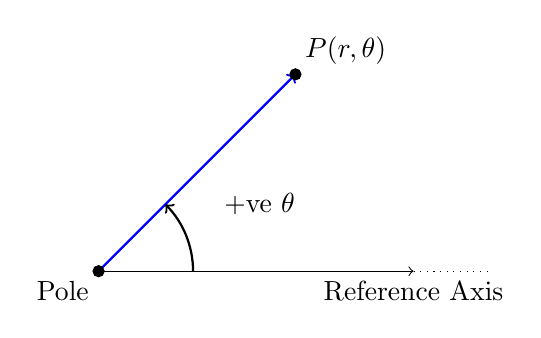
\begin{tikzpicture}
      \draw[->] (0,0) -- (4,0) node[anchor=north] {Reference Axis};
      \draw[dotted] (4,0) -- (5,0);
      \draw[->, thick, blue] (0,0) -- (2.5,2.5);
      \node at (2.5,2.5) [above right] {$P(r, \theta)$};
      \draw[->, thick] (0:1.2) arc[start angle=0, end angle=45, radius=1.2];
      \node at (30:1.7) [right] {+ve $\theta$};
      \filldraw[black] (0,0) circle (2pt) node[anchor=north east] {Pole};
      \filldraw[black] (2.5,2.5) circle (2pt);
    \end{tikzpicture}
    \caption{+ve $r$, +ve $\theta$ (standard)}
  \end{subfigure}
  \hfill

  % Case 2: r < 0, theta > 0
  \begin{subfigure}[b]{0.45\textwidth}
    \centering
    \begin{tikzpicture}
      \draw[->] (0,0) -- (4,0) node[anchor=north] {Reference Axis};
      \draw[dotted] (4,0) -- (5,0);
      \draw[->, thick, red] (0,0) -- (-2.5,-2.5);
      \node at (-2.5,-2.5) [below left] {$P(-r, \theta)$};
      \draw[->, thick] (0:1.2) arc[start angle=0, end angle=45, radius=1.2];
      \node at (30:1.7) [right] {+ve $\theta$};
      \filldraw[black] (0,0) circle (2pt) node[anchor=north east] {Pole};
      \filldraw[black] (-2.5,-2.5) circle (2pt);
    \end{tikzpicture}
    \caption{-ve $r$, +ve $\theta$ (point in opposite direction)}
  \end{subfigure}

  \vspace{1em}

  % Case 3: r > 0, theta < 0
  \begin{subfigure}[b]{0.45\textwidth}
    \centering
    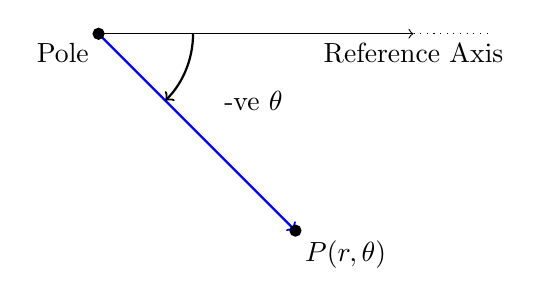
\begin{tikzpicture}
      \draw[->] (0,0) -- (4,0) node[anchor=north] {Reference Axis};
      \draw[dotted] (4,0) -- (5,0);
      \draw[->, thick, blue] (0,0) -- (2.5,-2.5);
      \node at (2.5,-2.5) [below right] {$P(r, \theta)$};
      \draw[->, thick] (0:1.2) arc[start angle=0, end angle=-45, radius=1.2];
      \node at (-30:1.7) [right] {-ve $\theta$};
      \filldraw[black] (0,0) circle (2pt) node[anchor=north east] {Pole};
      \filldraw[black] (2.5,-2.5) circle (2pt);
    \end{tikzpicture}
    \caption{+ve $r$, -ve $\theta$ (clockwise)}
  \end{subfigure}
  \hfill

  % Case 4: r < 0, theta < 0
  \begin{subfigure}[b]{0.45\textwidth}
    \centering
    \begin{tikzpicture}
      \draw[->] (0,0) -- (4,0) node[anchor=north] {Reference Axis};
      \draw[dotted] (4,0) -- (5,0);
      \draw[->, thick, red] (0,0) -- (-2.5,2.5);
      \node at (-2.5,2.5) [above left] {$P(-r,- \theta)$};
      \draw[->, thick] (0:1.2) arc[start angle=0, end angle=-45, radius=1.2];
      \node at (-30:1.7) [right] {-ve $\theta$};
      \filldraw[black] (0,0) circle (2pt) node[anchor=north east] {Pole};
      \filldraw[black] (-2.5,2.5) circle (2pt);
    \end{tikzpicture}
    \caption{-ve $r$, -ve $\theta$ (point in opposite direction)}
  \end{subfigure}

  \caption{All four sign combinations of polar coordinates with correct angle and direction of $r$}
  \label{fig:polar-corrected}
\end{figure}

The direction of +ve \( \theta \) is by convention counter-clockwise.\\
The direction of +ve \( r \) is by convention in the direction of theta.\\
So, the direction of -ve \( \theta \) is clockwise.\\
And, the direction of -ve \( r \) is in the opposite direction of \( \theta \).\\
So, if \( \theta \) is clockwise, \( r \) is in the clockwise direction and \( -r \) is in the counter-clockwise direction.\\

\section{Graphing Polar Equations or Inequalities}
\label{sec:graph-polar-equat-ineq}
Polar equations or Set of polar inequalities can be used to plot graphs of
usually circular figures.
\begin{note}
  Some special cases:\\
  \begin{enumerate}
    \item \(r=\left| a \right| \) gives a circle with center as pole and radius as \( a \).
    \item \( \theta=\theta_o \) gives a straight line passing through the pole.
    \item \sout{\( r=a\)} \(r=\left| a \right| \), \(\theta=\theta_o \) gives a
      point \( P(a,\theta_o) \).
  \end{enumerate}
\end{note}

\section{Examples of Polar Graphing}
\label{sec:examples-polar-graphing}

\begin{eg}[Plot the graph of: \( 1 \le r \le 2,\, 0 \le \theta \le \pi/2 \)]
  \label{eg:polar-graph-eg1}
\end{eg}
\begin{answer}
  \begin{center}
    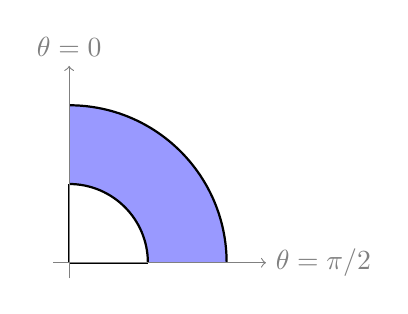
\begin{tikzpicture}
      \fill[blue!50, opacity=0.8]
        (0:1) arc (0:90:1) --
        (90:2) arc (90:0:2) --
        cycle;

      % Draw the boundary arcs and lines
      \draw[thick] (0:1) arc (0:90:1);
      \draw[thick] (0:2) arc (0:90:2);
      \draw[thick] (0,0) -- (0:1);
      \draw[thick] (0,0) -- (90:1);

      % Axes (optional)
      \draw[->, gray] (-0.2,0) -- (2.5,0) node[right] {\(\theta=\pi/2\)};
      \draw[->, gray] (0,-0.2) -- (0,2.5) node[above] {\(\theta=0\)};
    \end{tikzpicture}
  \end{center}
\end{answer}


\begin{eg}[Plot the graph of: \( -3 \le r \le 2,\, \theta = \pi/4 \)]
  \label{eg:polar-graph-eg2}
\end{eg}
\begin{answer}
  \begin{center}
    \begin{tikzpicture}
      \fill (0,0) circle (1pt);
      \draw[->, gray] (-4,0) -- (4,0) node[right] {\( \theta=0 \)};
      \draw[thick, ->] (0:1) arc (0:45:1);
      \draw[thick] (45:-3) -- (45:2);
      \node at (20:1.5) {\( \theta = \frac{\pi}{4}\)};
      \fill (225:3) circle (1.5pt) node[anchor=north east] {\( r = -3 \)};
      \fill (45:2) circle (1.5pt) node[anchor=south west] {\( r = 2 \)};
    \end{tikzpicture}
  \end{center}
\end{answer}

\begin{eg}[Plot the graph of: \( \frac{\pi}{3} \le \theta \le \frac{5\pi}{6} \)]
  \label{eg:polar-graph-eg3}
\end{eg}
\begin{answer}
  \begin{center}
    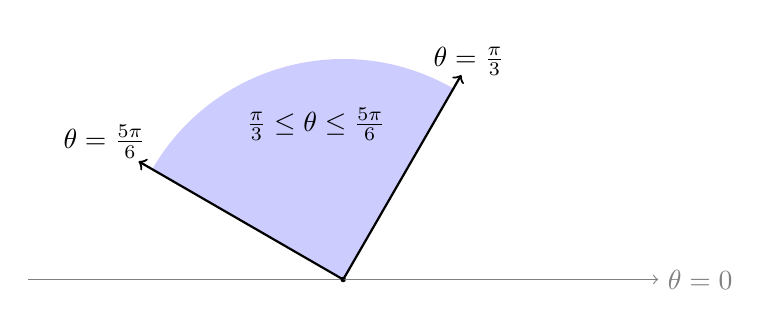
\begin{tikzpicture}
      \fill[blue!20] (0,0) -- (60:2.8) arc (60:150:2.8) -- cycle;
      \fill (0,0) circle (1pt);
      \draw[->, gray] (-4,0) -- (4,0) node[right] {\( \theta=0 \)};
      \node at (100:2) {\( \frac{\pi}{3} \le \theta \le \frac{5\pi}{6} \)};
      \draw[thick, ->] (60:0) -- (60:3);
      \draw[thick, ->] (150:0) -- (150:3);
      \node at (60:3.2) {\( \theta = \frac{\pi}{3} \)};
      \node at (150:3.5) {\( \theta = \frac{5\pi}{6} \)};
    \end{tikzpicture}
  \end{center}
\end{answer}

\section{Exercise 1}\label{ex:polar-coords-ex1}

\begin{exercise}
  \textbf{Plot the graph of the following:}
  \begin{enumerate}
    \item \( r \ge 1 \)
      \begin{answer}
        \begin{center}
          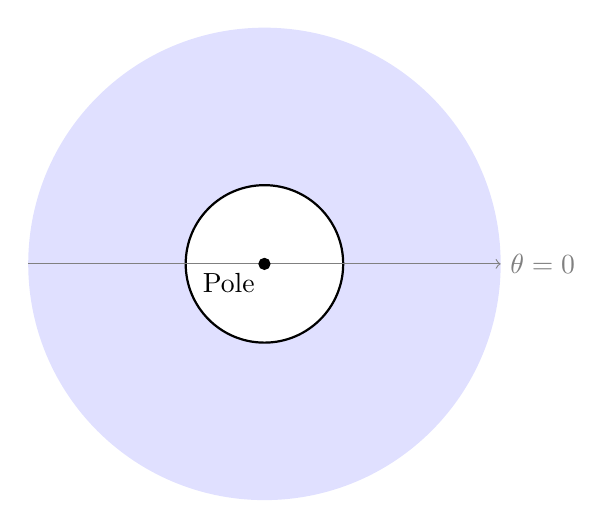
\begin{tikzpicture}
            \fill[blue!20, opacity=0.6] (0,0) circle (3);
            \fill[white] (0,0) circle (1);
            \draw[thick] (0,0) circle (1);
            \draw[->, gray] (-3,0) -- (3,0) node[right] {\( \theta=0 \)};
            \filldraw[black] (0,0) circle (2pt) node[anchor=north east] {Pole};
          \end{tikzpicture}
        \end{center}
      \end{answer}

    \item \( 1 \le r \le 2 \)
      \begin{answer}
        \begin{center}
          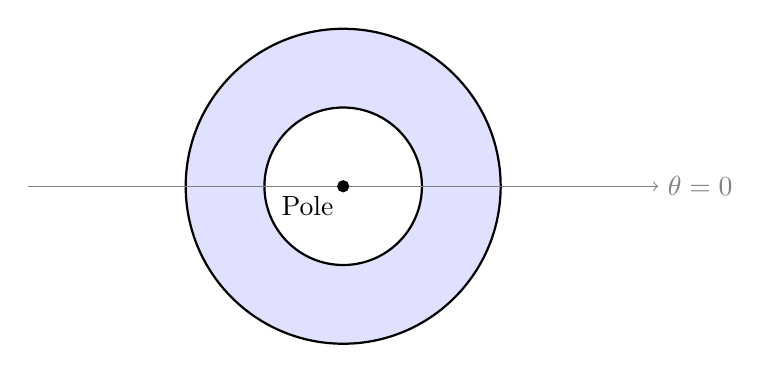
\begin{tikzpicture}
            \fill[blue!20, opacity=0.6] (0,0) circle (2);
            \fill[white] (0,0) circle (1);
            \draw[thick] (0,0) circle (1);
            \draw[thick] (0,0) circle (2);
            \draw[->, gray] (-4,0) -- (4,0) node[right] {\( \theta=0 \)};
            \filldraw[black] (0,0) circle (2pt) node[anchor=north east] {Pole};
          \end{tikzpicture}
        \end{center}
      \end{answer}

    \item \( 0 \le \theta \le \pi/2 \), \( 1 \le r \le 2 \)
      \begin{answer}
        \begin{center}
          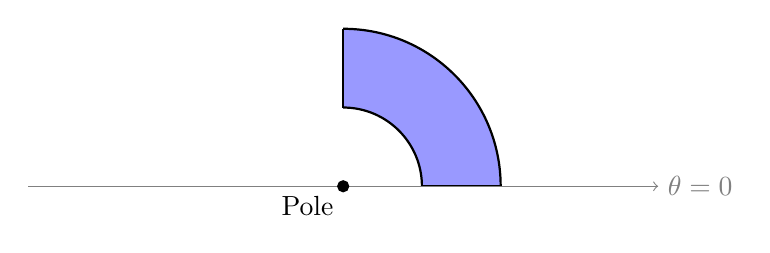
\begin{tikzpicture}
            \fill[blue!50, opacity=0.8]
              (0:1) arc (0:90:1) --
              (90:2) arc (90:0:2) --
              cycle;
            \draw[thick] (0:1) arc (0:90:1);
            \draw[thick] (0:2) arc (0:90:2);
            \draw[thick] (1,0) -- (0:2);
            \draw[thick] (0,1) -- (90:2);
            \draw[->, gray] (-4,0) -- (4,0) node[right] {\( \theta=0 \)};
            \filldraw[black] (0,0) circle (2pt) node[anchor=north east] {Pole};
          \end{tikzpicture}
        \end{center}
      \end{answer}

    \item \( 0 \le \theta \le \pi/6 \), \( r \ge 0 \)
      \begin{answer}
        \begin{center}
          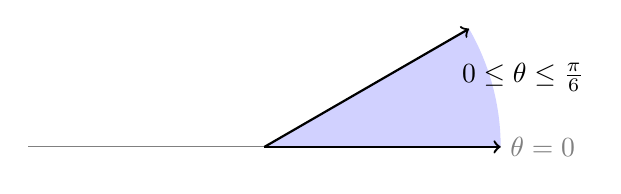
\begin{tikzpicture}
            \fill[blue!30, opacity=0.6] (0,0) -- (0:3) arc (0:30:3) -- cycle;
            \draw[->, gray] (-3,0) -- (3,0) node[right] {\( \theta = 0 \)};
            \draw[thick, ->] (0,0) -- (0:3);
            \draw[thick, ->] (0,0) -- (30:3);
            \node at (15:3.4) {\( 0 \le \theta \le \frac{\pi}{6} \)};
          \end{tikzpicture}
        \end{center}
      \end{answer}

    \item \( \theta=\pi/2 \), \( r \le 0 \)
      \begin{answer}
        \begin{center}
          \begin{tikzpicture}
            \draw[->, thick] (0,0) -- (270:3);
            \draw[->, gray] (-3,0) -- (3,0) node[right] {\( \theta = 0 \)};
            \draw[->, gray] (0,-3) -- (0,3) node[above] {\( \theta = \frac{\pi}{2} \)};
            \node at (90:-3.2) {-ve y-axis};
          \end{tikzpicture}
        \end{center}
      \end{answer}

    \item \( \theta=\pi/2 \), \( r \ge 0 \)
      \begin{answer}
        \begin{center}
          \begin{tikzpicture}
            \draw[->, thick] (0,0) -- (90:3);
            \draw[->, gray] (0,0) -- (3,0) node[right] {\( \theta = 0 \)};
            \node at (90:3.2) {+ve y-axis};
          \end{tikzpicture}
        \end{center}
      \end{answer}

    \item \( -\pi/2 \le \theta \le \pi/2 \), \( 1 \le r \le 2 \)
      \begin{answer}
        \begin{center}
          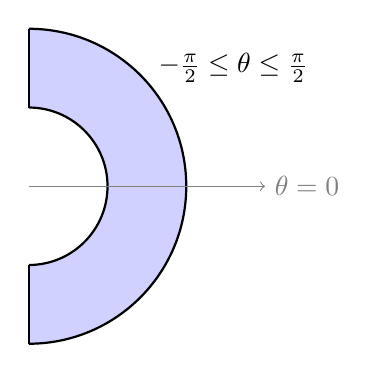
\begin{tikzpicture}
            \fill[blue!30, opacity=0.6]
              (-90:1) arc (-90:90:1) --
              (90:2) arc (90:-90:2) -- cycle;
            \draw[thick] (-90:1) arc (-90:90:1);
            \draw[thick] (-90:2) arc (-90:90:2);
            \draw[thick] (0,-1) -- (-90:2);
            \draw[thick] (0,1) -- (90:2);
            \node at (30:3) {\( -\frac{\pi}{2} \le \theta \le \frac{\pi}{2} \)};
            \draw[->, gray] (0,0) -- (3,0) node[right] {\( \theta = 0 \)};
          \end{tikzpicture}
        \end{center}
      \end{answer}

  \end{enumerate}
\end{exercise}
